\documentclass[]{beamer}
% Class options include: notes, notesonly, handout, trans,
%                        hidesubsections, shadesubsections,
%                        inrow, blue, red, grey, brown
\usepackage{graphicx}
\usepackage{hyperref}
\usepackage{fancyvrb}
\usepackage{subfig}

\usepackage[utf8]{inputenc}
\usepackage[spanish]{babel}
\usepackage[style=authoryear]{biblatex}
\renewcommand*{\nameyeardelim}{\addcomma\addspace}

\uselanguage{Spanish}
\languagepath{Spanish}

% Theme for beamer presentation.
\usepackage{beamerthemesplit} 
% Other themes include: beamerthemebars, beamerthemelined, 
%                       beamerthemetree, beamerthemetreebars  
% \usetheme{Warsaw}
% \usetheme{Rochester}
\usetheme{Boadilla}

\setbeamertemplate{headline}{%
\leavevmode%
  \hbox{%
    \begin{beamercolorbox}[wd=\paperwidth,ht=2.5ex,dp=1.125ex]{palette quaternary}%
    \insertsectionnavigationhorizontal{\paperwidth}{}{\hskip0pt plus1filll}
    \end{beamercolorbox}%
  }
}

\title[CeCAR]{Utilizando el CeCAR}
% \subtitle{Tesis presentada para optar al título de Doctor de la Universidad de Buenos Aires en el área Ciencias de la Computación}
\author[Saveli Vassiliev]{Saveli Vassiliev}
\institute[UBA, FCEyN, IC]{Universidad de Buenos Aires \\ Facultad de Ciencias Exactas y Naturales, Instituto de Cálculo}
\date{\today}                    % Enter the date or \today between curly braces

\begin{document}

% Creates title page of slide show using above information
\begin{frame}
  \titlepage
\end{frame}

%\section[Outline]{}
%
%% Creates table of contents slide incorporating
%% all \section and \subsection commands
%\begin{frame}
%  \tableofcontents
%\end{frame}


\begin{frame}
\frametitle{Plan}
\begin{itemize}
  \item Creación de claves y usuarios. Usaremos \Verb=PuTTY= para conectarnos al cluster y \Verb=WinSCP= para mover archivos.
  \item Introducción a la terminal de Linux necesario para ejecutar aplicaciones.
  \item Introducción a comandos de control de \Verb=Slurm=
\end{itemize}
\end{frame}

\begin{frame}
\frametitle{Para usuarios de Windows}
\begin{itemize}
  \item CeCAR es un cluster de exactas, físicamente en el pabellón 1.
  \item Utiliza SLURM para controlar ejecución de trabajos.
  \item Hay que saber comandos básicos de linux y algún gestor de 
  \end{itemize}
\end{frame}

\begin{frame}
\frametitle{Para usuarios de Windows}
\begin{enumerate}
  \item Descargar y instalar PuTTY de \url{https://www.putty.org/}
  \item Abrir \Verb=<Archivos de programa>/puttygen.exe=
  \item Clickear en \Verb=Generate= (esto genera un par de claves, la pública y la privada).
  \item Poner un nombre que les permita recordar qué computadora usan en \Verb=Key comment= (sin espacios).
\end{enumerate}
  \begin{center}
  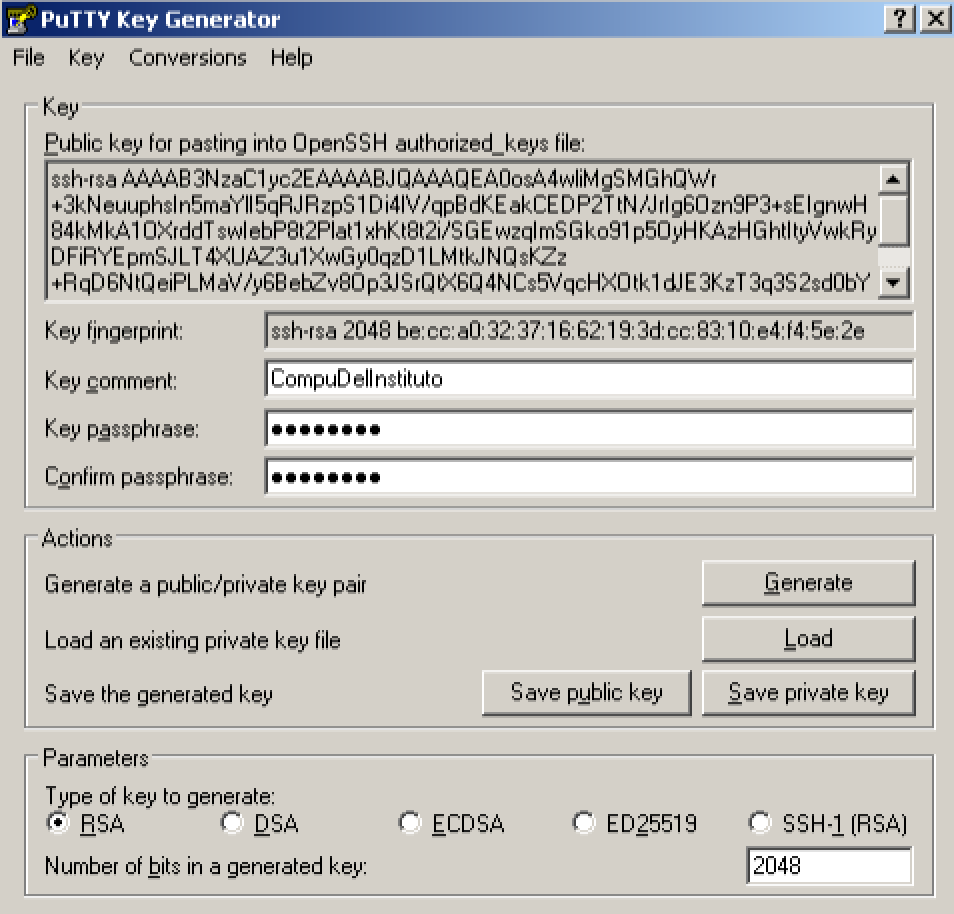
\includegraphics[width=13em]{./puttygen}
  \end{center} 
\end{frame}

\begin{frame}
\begin{enumerate}
  \item Escribir un passphrase (una contraseña suya).
  \item Guardar la clave privada en un archivo \Verb=cecar.ppk=
  \item Copiar la clave generada a la web del CeCAR como sigue.
\end{enumerate}
\begin{center}
  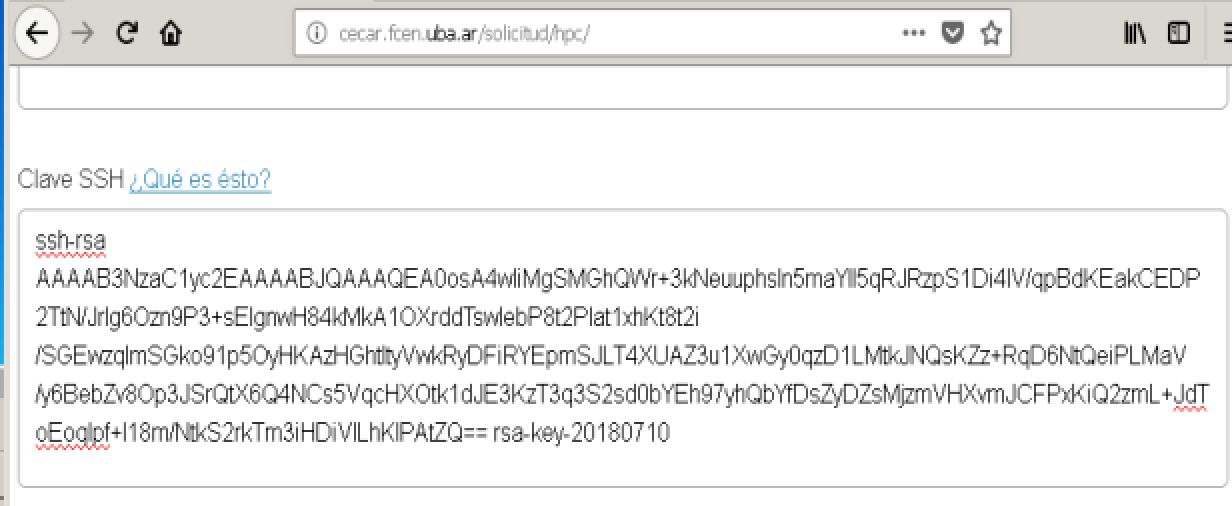
\includegraphics[width=23em]{./ssh-web-cecar}
  \end{center} 
\end{frame}


\begin{frame}
\begin{enumerate}
  \item Descargar e instalar \Verb=WinSCP= de \url{https://winscp.net/}
  \item lalala
\end{enumerate}
\begin{center}
  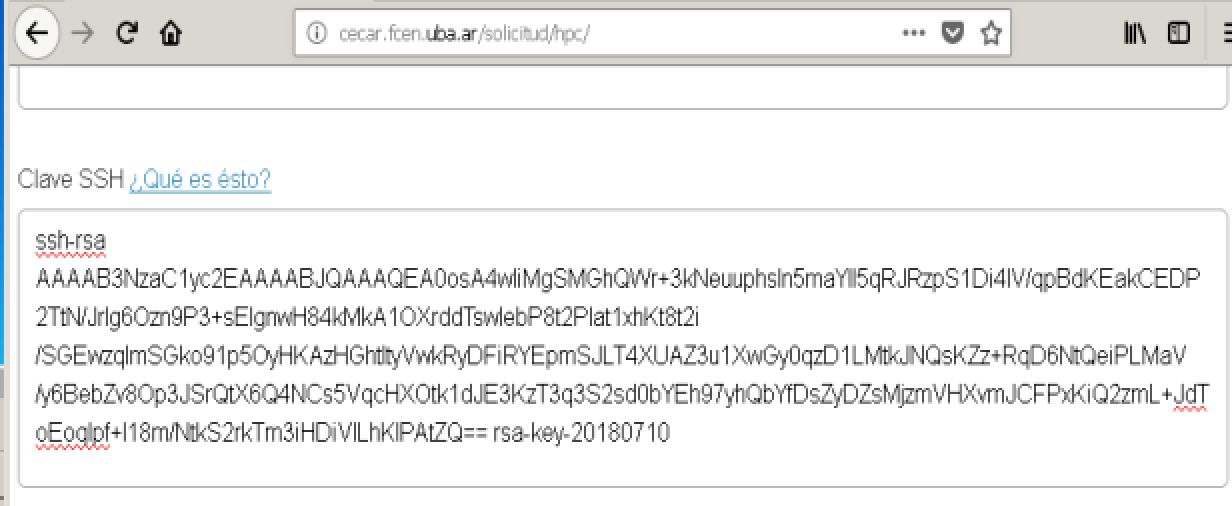
\includegraphics[width=23em]{./ssh-web-cecar}
  \end{center} 
\end{frame}



\begin{frame}
\frametitle{Cliques}
 \begin{definition}[Clique]
 Una \emph{clique} es un subgrafo completo \textbf{maximal} de $G$. Ejemplo:
 \end{definition}
\end{frame}

\begin{frame}[allowframebreaks]{References}
\def\newblock{}
% \printbibliography
% \bibliographystyle{alpha}
% \bibliography{../thesis/references}
\end{frame}


\end{document}